% Hinweis: Optionen der Dokumentenklasse werden an alle folgenden \usepackage{package} Befehle weitergegeben
\documentclass[
	pdftex,
	fontsize=12pt,
	paper=a4,
	halfparskip,
	twoside=false,
	numbers=noenddot,	% Kein Punkt am Ende einer Überschrift
	%draft=true,			% Deckt Schwächen auf: overfull und full boxes werden markiert; Bilder werden nicht geladen
	bibliography=totoc,	% Literaturverzeichnis ins Inhaltsverzeichnis aufnehmen
	listof=totoc,		% Tabellen- und Abbildungsverzeichnis ins Inhaltsverzeichnis aufnehmen
	titlepage=true,		% Separate Titelseite; Gestaltung mit Hilfe der Titlepage-Umgebung
	headsepline=true,	% Kopflinie aktivieren
	footsepline=true	,	% Fußlinie aktivieren
	abstracton			% Abstract aktivieren
]{scrreprt}

% Zeichenkodierung Input ist UTF-8: Umlaute können direkt eingegeben werden
\usepackage[utf8]{inputenc}

% Zeichenkodierung Ausgabe ist T1-Kodierung: Wichtig für die Ausgabe von Umlauten
\usepackage[T1]{fontenc}

% Schrift festlegen
\usepackage{lmodern}

% Sprachauswahl für Lokalisierungen und Silbentrennung
\usepackage[ngerman]{babel}

% Zitate: Anführungszeichen automatisch anhand der Sprache wählen
\usepackage[babel=true]{csquotes}

% Source-Code-Listings
\usepackage{listings}

% BibTeX-Symbol
\usepackage{texnames}

\usepackage{xcolor}

% Symbole, z.B. Haken
\usepackage{pifont}

% Zeilen in Tabellen zusammenfassen
\usepackage{multirow}

% Silbentrennung kann bei bestimmten Wörten mit Hilfe von diesem Paket deaktiviert werden 
\usepackage{hyphenat}

% Abkürzungsverzeichnis
%\usepackage[printonlyused, withpage]{acronym}
% Abstand mit Punkten füllen
%\renewcommand*\aclabelfont[1]{\textbf{\normalsize{#1}}\hfill}

% Tiefe des Inhaltsverzeichnisses
\setcounter{tocdepth}{2}

% Punkte im Inhaltsverzeichnis
\usepackage{tocstyle}
\usetocstyle{allwithdot}

% Zum Einbinden von PDF-Dateien.
\usepackage{pdfpages}

% Paket zum Anpassen von Kopf- und Fußzeilen
\usepackage[plainfootsepline, plainheadsepline, headsepline, footsepline, automark]{scrpage2}
% Liniendicke
\setheadsepline{0.1pt}
\setfootsepline{0.1pt}

% Kopf- und Fusszeile löschen
\clearscrheadfoot
% Kopf- und Fusszeile aktivieren
\pagestyle{scrheadings}

% Kopf links
\ihead[\titel]{\titel}

% Fuss links
\ifoot[\verfasser]{\verfasser}
% Fuss rechts
\ofoot[\pagemark]{\pagemark}

% Grafiken einbinden
\usepackage{graphicx}
% Pfad zu den Grafiken
\graphicspath{{Abbildungen/}}

% Seitenränder setzen
\usepackage[left=3cm, right=2cm, top=2.5cm, bottom=3cm]{geometry}

% Zeilenabstand auf 1.5 setzen
\usepackage{setspace}
\onehalfspacing

% Literaturverzeichnis
%\usepackage[backend=bibtex,style=authoryear]{biblatex}
%\usepackage{bibgerm}
%\usepackage{natbib}
\usepackage[backend=bibtex,style=alphabetic]{biblatex}
%\bibliographystyle{alphadin}
\bibliography{Literatur/Literatur.bib}

% Glossar
\usepackage[toc,nonumberlist]{glossaries}

% Titel als Referenzierung verwenden
\usepackage{titleref}

% Währungen
\usepackage{textcomp}

% Fussnoten fortlaufend nummerieren.
\usepackage{chngcntr}
\counterwithout{footnote}{chapter}

% Persönliche Daten
\newcommand{\titel}{Lerntheorien: Kognitivismus, Konstruktivismus und Konnektivismus}
\newcommand{\untertitel}{}
\newcommand{\art}{Seminararbeit}
\newcommand{\verfasser}{Alexander Hauck und Fabian Berns}
\newcommand{\kurs}{WWI13B5}
\newcommand{\ausbildungsbetrieb}{SAP SE}%, Dietmar-Hopp-Allee 16, 69190 Walldorf}
\newcommand{\abgabedatum}{__________________}

\newcommand{\martrikelnr}{}
\newcommand{\betreuer}{Frau Judith Hüther}
\newcommand{\gutachter}{}
\newcommand{\zeitraum}{November 2015 - Januar 2016}


% Links- und PDF-Einstellungen
\usepackage{hyperref}
\hypersetup{
	pdfauthor = {\verfasser},
	pdftitle = {\titel},
	pdfsubject = {\art},
	pdfkeywords = {},
	pdfstartview = {Fit},
	colorlinks = {false},
	breaklinks = {true},
	bookmarksopen = {true}
}

% Verhinderung von Schusterjunge und Hurenkind
\clubpenalty = 10000
\widowpenalty = 10000
\displaywidowpenalty = 10000

% Seitenzäler für große, römische Zahlen
\newcounter{RomanPagenumber}

% Abkürzungen
\newcommand{\dash}{d.\,h.}
\newcommand{\zB}{z.\,B.}

%Für Javascript Code
\usepackage{color}
\definecolor{lightgray}{rgb}{.9,.9,.9}
\definecolor{darkgray}{rgb}{.4,.4,.4}
\definecolor{purple}{rgb}{0.65, 0.12, 0.82}

\lstdefinelanguage{JavaScript}{
	keywords={typeof, new, true, false, catch, function, return, null, catch, switch, var, if, in, while, do, else, case, break},
	keywordstyle=\color{blue}\bfseries,
	ndkeywords={class, export, boolean, throw, implements, import, this},
	ndkeywordstyle=\color{darkgray}\bfseries,
	identifierstyle=\color{black},
	sensitive=false,
	comment=[l]{//},
	morecomment=[s]{/*}{*/},
	commentstyle=\color{purple}\ttfamily,
	morestring=[b]',
	morestring=[b]",
}

\begin{document}
	% Titelseite
	\thispagestyle{plain}

\begin{titlepage}
	
	%\begin{longtable}{p{.55\textwidth} p{.85\textwidth}}
	%{
\includegraphics[height=2.4cm]{Abbildungen/SAP_grad_R_min}}&
	\centering
\includegraphics[height=3cm]{Abbildungen/dhbw}	
	%\end{longtable}
	\enlargethispage{20mm}
	
	\begin{center}
		\vspace*{12mm}	{\LARGE\bf \titel }\\
		\vspace*{12mm}	{\large\bf \art}\\
		\vspace*{12mm}	im Rahmen der Prüfung zum\\
		\vspace*{3mm} 	\textbf{Bachelor of Science (B.\,Sc.)}\\
		\vspace*{12mm}	des Studienganges Wirtschaftsinformatik (Sales und Consulting)\\
		\vspace*{3mm} 	an der Dualen Hochschule Baden-Württemberg Karlsruhe\\
		\vspace*{12mm}	von\\
		\vspace*{3mm} 	{\large\bf \verfasser}\\
		%\vspace*{12mm}	{\abgabedatum}\\
		%\vspace*{3mm}     -- Sperrvermerk --\\
		
	\end{center}
	\vfill
	\begin{spacing}{1.7}
		\begin{center}\parbox{0cm}{
				\begin{tabbing}
					mmmmmmmmmmmmmmmmmmmmm \=  \kill
					%\textbf{Bearbeitungszeitraum}  \>  \zeitraum\\
					\textbf{Kurs}  				   \>  \kurs\\
					\textbf{Ausbildungsfirma}      \>  \ausbildungsbetrieb\\
					\textbf{Betreuer}              \>  \betreuer\\
					\textbf{Abgabedatum}		   \>  11.01.2016 
				\end{tabbing}
			}
		\end{center}
	\end{spacing}
	\vfill
\end{titlepage}
	
	% Ab hier große, römische Seitenzahlen
	\pagenumbering{Roman}
	
	% Sperrvermerk
	%\addchap{Sperrvermerk}
Die nachfolgende Arbeit enthält vertrauliche Daten und Informationen der SAP Deutschland SE \& Co. KG.
Veröffentlichungen oder Vervielfältigungen -- auch nur auszugsweise -- sind ohne ausdrückliche schriftliche Genehmigung des Unternehmens nicht gestattet.

Die Arbeit ist nur den Korrektoren sowie den Mitgliedern des Prüfungsausschusses zugänglich zu machen.
Über den Inhalt ist Stillschweigen zu bewahren.
	
	% Eidesstattliche Erklärung
	\addchap{Eidesstattliche Erklärung}
Wir versichern hiermit, dass wir diese Seminararbeit mit dem Thema: \emph{\titel} selbstständig verfasst und keine anderen als die angegebenen Quellen und Hilfsmittel benutzt habe. Wir versichern zudem, dass die eingereichte elektronische Fassung mit der gedruckten Fassung übereinstimmt.

Diese Arbeit wurde bisher in gleicher oder ähnlicher Form oder auszugsweise noch keiner Prüfungsbehörde vorgelegt und auch nicht veröffentlicht.
\\
\vspace{2cm}
\\
\underline{\hspace{5cm}}\\
\noindent (Alexander Hauck)
\\
\noindent Karlsruhe, den 11.01.2016

\leavevmode
\vspace{2cm}
\\
\underline{\hspace{5cm}}\\
\noindent (Fabian Berns)
\\
\noindent Karlsruhe, den 11.01.2016
	
	%Abstract
	%\pagestyle{empty}

\renewcommand{\abstractname}{Zusammenfassung}
\begin{abstract}
Ein Abstract ist eine prägnante Inhaltsangabe, ein Abriss ohne
Interpretation und Wertung einer wissenschaftlichen Arbeit. In DIN
1426 wird das (oder auch der) Abstract als Kurzreferat zur
Inhaltsangabe beschrieben.

\begin{description}
\item[Objektivität] soll sich jeder persönlichen Wertung enthalten
\item[Kürze] soll so kurz wie möglich sein
\item[Genauigkeit] soll genau die Inhalte und die Meinung der Originalarbeit wiedergeben
\end{description}

Üblicherweise müssen wissenschaftliche Artikel einen Abstract
enthalten, typischerweise von 100-150 Wörtern, ohne Bilder und
Literaturzitate und in einem Absatz.

Quelle \url{http://de.wikipedia.org/wiki/Abstract} Abgerufen 07.07.2011
\end{abstract}


\renewcommand{\abstractname}{Summary}
\begin{abstract}
An abstract is a brief summary of a research article, thesis, review,
conference proceeding or any in-depth analysis of a particular subject
or discipline, and is often used to help the reader quickly ascertain
the paper's purpose. When used, an abstract always appears at the
beginning of a manuscript, acting as the point-of-entry for any given
scientific paper or patent application. Abstracting and indexing
services for various academic disciplines are aimed at compiling a
body of literature for that particular subject.

The terms précis or synopsis are used in some publications to refer to
the same thing that other publications might call an "abstract". In
management reports, an executive summary usually contains more
information (and often more sensitive information) than the abstract
does.

Quelle: \url{http://en.wikipedia.org/wiki/Abstract_(summary)}

\end{abstract}

	
	% Inhaltsverzeichnis
	\tableofcontents
	\pagebreak
	
	% Abbildungsverzeichnis
	\listoffigures
	\pagebreak
	
	% Tabellenverzeichnis
	%\listoftables
	%\pagebreak
	
	% Abkürzungsverzeichnis
	%\addchap{Abkürzungsverzeichnis}
	%% Alle Abkürzungen hier definieren.
% Alphabetische Sortierung ist von Hand vorzunehmen.
\begin{acronym}[HTTPS] % Längstes Akronym in eckigen Klammern
	% Kein Abstand, kompakte Darstellung
	%\setlength{\itemsep}{-\parsep} 
	%A
	%B
	%C
	%D
	%E
	%F
	%G
	%H
	\acro{HTTPS}{Hypertext Transfer Protocol Secure}
	%I
	%J
	%K
	%L
	%M
	%N
	%O
	%P
	%Q
	%R
	%S
	\acro{SAP}{Sack aus Plaste}
	%T
	%U
	%V
	%W
	%X
	%X
	%Y
	%Z	
\end{acronym}
	%\pagebreak
	
	% Abschnitt beenden
	\clearpage
	
	% Seitenzähler erhält den Wert der aktuellen groß römisch nummerierten Seite; Zwischenspeichern für später
	\setcounter{RomanPagenumber}{\value{page}}
	
	% Ab hier arabische Seitenzahlen
	\pagenumbering{arabic}
		
	% Kopf links auf aktuelles Kapitel ändern
	\automark{chapter}
	\ihead[\headmark]{\headmark}	
	\renewcommand*{\chaptermarkformat}{}	
	
	% Inhalt der Arbeit
	%\chapter{Beispiele}
\label{cha:Beispiele}

\section{Zitieren}

\enquote{Ich bin ein direktes Zitat} nach \citeauthor{Nachname.2013} aus \cite[42]{.2000}.

\enquote{Ich bin ein direktes Zitat} nach \citeauthor{Glover.2006} aus \cite[42]{Glover.2006}.
\section{Verweise}

\autoref{cha:Beispiele} zeigt ab Seite~\pageref{cha:Beispiele} Beispiele zur Syntax von \LaTeX{}.

Titel zitieren: \citetitle{Nachname.2013}

\section{Aufzählungen}
\label{sec:Aufzaehlungen}

\subsection{Itemize}

\begin{itemize}
	\item
		Ich bin das erste Item
	\item
		Ich bin das zweite Item.
\end{itemize}description

\subsection{Enumerate}

\begin{enumerate}
	\item
		Ich bin das erste Item
	\item
		Ich bin das zweite Item.
\end{enumerate}

\subsection{Description}

\begin{description}
	\item[Item 1]
		Ich bin das erste Item
	\item[Item 2]
		Ich bin das zweite Item.
\end{description}

\section{Abbildungen}

In \autoref{fig:LogoDHBW Karlsruhe} auf Seite~\pageref{fig:LogoDHBW Karlsruhe} ist das Logo der DHBW Karlsruhe zu sehen.

\begin{figure}[!htbp]
	\centering
	
\includegraphics[scale=0.75]{Abbildungen/Logo_DHBW_Karlsruhe.png}
	\caption{Logo der DHBW Karlsruhe}
	\label{fig:LogoDHBW Karlsruhe}
\end{figure}

\section{Tabellen}

Tabelle~\ref{tbl:TestTabelle} auf Seite~\pageref{tbl:TestTabelle} zeigt eine Test-Tabelle.

\begin{table}[!htbp]
	\centering
	\begin{tabular}{ll}
		\textbf{Test}	& \textbf{Test}\\
		\hline
		Test 	&	Test\\
		Test 	&	Test\\
		\hline
	\end{tabular}
	\caption{Test-Tabelle}
	\label{tbl:TestTabelle}
\end{table}

\begin{table}[!htbp]
	\centering
	\begin{tabular}{ll}
		\textbf{Test}	& \textbf{Test}\\
		\hline
		Test 	&	Test\\
		Test 	&	Test\\
		\hline
	\end{tabular}
	\caption{Test-Tabelle 2}
	\label{tbl:TestTabelle2}
\end{table}

\section{Abkürzungen}

\ac{T} ist eine Abkürzung.
\ac{T} wird beim ersten Vorkommen zur Erklärung ausgeschrieben.

Und noch eine Abkürzung: \ac{TT}.
	\chapter{Einleitung}
\label{cha:Einleitung}
In dieser Seminararbeit wird das Thema Lerntheorien mit speziellem Bezug auf die Theorien Kognitivismus, Konstruktivismus und Konnektivismus behandelt. Diese Arbeit entstand im Zeitraum November 2015 bis Januar 2016 im Zuge des Integrationsseminar zu ausgewählten Themen der Wirtschaftsinformatik im fünften Semester. In dieser Einleitung wird zu Beginn auf das zentrale Thema dieser Arbeit, den Lerntheorien, und im Anschluss auf die Modelle didaktischer Aufbereitung eingegangen. Auf letzteren liegt zwar nicht der Fokus dieses Textes, die Autoren geben jedoch, neben den allgemeinen Lerntheoriedefinitionen sowie Anwendungshinweisen bzgl. E-Learning-Instrumenten für jede der drei Theorien (vgl. Kapitel 2 - 4), Hinweise darüber, welches didaktisches Modell welcher Lerntheorie zugeordnet werden kann (siehe abschließendes Kapitel \ref{cha:Schluss}). 

\section{Lerntheorie}
\label{sec:Lerntheorie}
Lerntheorien befassen sich mit den in Theorien oder gar Gesetzmäßigkeiten gegossenen Ergebnissen aus Experimenten zur Erforschung von Lernen und Gedächtnis. Lernen wird von Irle als der Prozess des Informationserwerbs bezeichnet und wird von ihr abgegrenzt gegen das Gedächtnis. Dieses stehe für die Speicherung und Reproduzierung des Erlernten. \cite{Irle.1986}

Lerntheorien beschäftigen sich also damit, wie ein Mensch lernt. \cite{Reinmann.2013} Es existieren einige Lerntheorien, aber es gibt zur Zeit in der Wissenschaft keine etablierte Ansicht über das Zusammenspiel dieser, da sie oft als konkurrierend angesehen werden. \cite[S. 172 f.]{Weinert.1996} Dieses konkurrierende System an Lerntheorien löst sich aber perspektivisch auf \cite{WittKerres.2002} und man geht dazu über Lerntheorien themen- bzw. zweckbezogen gegeneinander aufzuwiegen. \cite{Reinmann.2013}

Dieses Aufwiegen der Lerntheorien gegeneinander bedeutet, dass der Lehrende je nach zu übermittelndem Inhalt bestimmt, gemäß welcher Lerntheorie die Lernenden das Wissen aufnehmen werden und sollen. Daraus kann dieser ableiten, wie er den Lernstoff didaktisch aufbereiten muss. Dazu gibt es zwei vorherrschende Modelle nach \cite{Kerres.2001}, welche im Folgenden beleuchtet werden. 

\section{Modelle didaktischer Aufbereitung}
\label{sec:Lernmodelle}
Bevor der Lernende Wissen aufnehmen kann, muss dieses erst aufbereitet werden und so 'zu ihm hingebracht' werden. Dies findet über Lehrmedien statt. Über die Art und Weise der Erstellung dieser Lehrmedien und darüber, welche Funktion diese genau haben sollen, gibt es unterschiedliche Auffassungen.

\subsection{Kopiermodell}
\label{sub:Kopiermodell}
\begin{figure}[h]
	\centering
	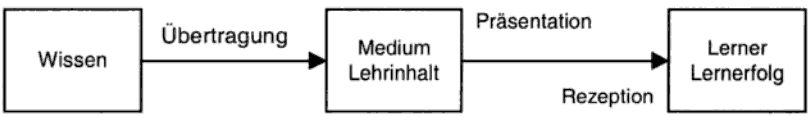
\includegraphics[width=0.7\textwidth]{Abbildungen/Kerres2001_Kopiermodell.PNG}
	\caption{Medien als Übermittler von Lehrinhalten. \cite[S. 146]{Kerres.2001}}
	\label{fig:Kerres2001_Kopiermodell}
\end{figure}
Gemäß dem Kopiermodell (siehe Graphik \ref{fig:Kerres2001_Kopiermodell})wird das zu erlernende "Wissen von Sachexpert/innen auf ein Medium übertragen werden und von da aus dem Lernenden präsentiert" \cite[S. 146]{Kerres.2001}. Dies führt zu der Annahme, dass das Medium und nicht der Lehrende präsentiert. Außerdem impliziert es die Gleichheit von Lehr- und Wissensinhalten.

Der Name Kopiermodell rührt daher, dass nach diesem didaktischen Modell Lernen nur das Kopieren von Wissen in das Gedächtnis darstellt und eine derartige 1:1 Kopie möglich und sinnvoll ist. \cite[S. 145 f.]{Kerres.2001}

\subsection{Lernen durch Anregung}
\label{sub:LernenDurchAnregung}
\begin{figure}[h]
	\centering
	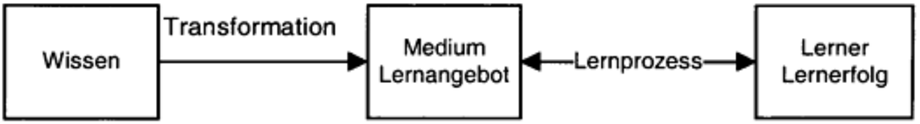
\includegraphics[width=0.7\textwidth]{Abbildungen/Kerres2001_LernenDurchAnregung.PNG}
	\caption{Medien als Angebot zur Anregung von Lernprozessen . \cite[S. 147]{Kerres.2001}}
	\label{fig:Kerres2001_LernenDurchAnregung}
\end{figure}
Das Kopiermodell gilt aufgrund neuer Erkenntnisse über die menschliche Art zu Lernen und Informationen aufzunehmen als veraltet.
In dem nun beschriebenen alternativen Modell sollen die Lernmedien vielmehr das aktive Lernen anregen, als nur die Lerninhalte wiedergeben. 
Dazu soll das zu vermittelnde Wissen eben in diese anregende Form transformiert werden. (siehe Graphik \ref{fig:Kerres2001_LernenDurchAnregung}) Diese Form soll neben der einfachen Aufnahme des Wissens auch zur Interaktion mit Mitlernenden und zur eigenen Aktion aufrufen. Beides soll die Intensität der Auseinandersetzung mit dem Lernstoff erhöhen. \cite[S. 147 f.]{Kerres.2001}
	\chapter{Kognitivismus}
\label{cha:Kognitivismus}
%Nachdem die beiden Abschnitte \ref{sub:Kopiermodell} und \ref{sub:LernenDurchAnregung} grundlegende Darstellungen der allgemeinen didaktischen Aufbereitung von Wissen mit Hilfe zweier Modelle gezeigt hat, beschreibt dieses Kapitel die Lerntheorie des Kognitivismus.%

\section{Definition}\label{Definition Kognitivismus}

Diese in den 60-er Jahren des letzten Jahrhunderts entwickelte Theorie beschreibt anders als die bis dahin vorherrschende behavioristische Lerntheorie nicht ausschließlich das Ergebnis des Lernprozesses, sondern die bis dahin als 'Black Box' verstandene Verarbeitung sowie Strukturierung von Wissen im Gehirn des Menschen. \cite[S. 155]{Erpenbeck.2007} 
Weiter kann der Kognitivismus als die Theorie beschrieben werden, welche die \textbf{Wahrnehmungs-}, \textbf{Denk-}, \textbf{Verstehens-}, sowie \textbf{Denkprozesse} näher betrachtet. Hierbei wird der Mensch als Informationsverarbeitungseinheit betrachtet. Er funktioniert ähnlich wie das aus der elektronischen Datenverarbeitung bekannte Datenverarbeitungsprinzip \textbf{EVA} (Eingabe, Verarbeitung, Ausgabe), wobei der Forschungsfokus dieser Theorie auf der Verarbeitung liegt. Folgende Abbildung verdeutlicht diese zusätzlich. \cite{AnsgarA.PlassmannProf.Dr.GunterSchmitt.2007}

\begin{figure}[h]
	\centering
	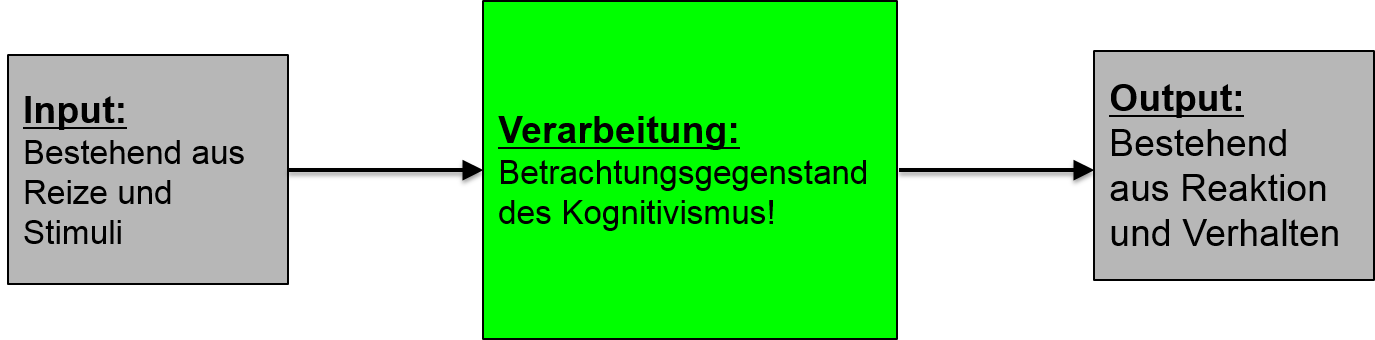
\includegraphics[width=0.9\textwidth]{Abbildungen/Kognitivismus1.PNG}
	\caption{Kognitivismus als EVA-Darstellung. In Anlehnung an \cite[S. 12]{SusanneMeir.}}
	\label{fig:Kerres2001_Kopiermodell}
\end{figure}

\section{Lernregeln des Kognitivismus sowie die Anwendung im E-Learning}

Folgende fünf kognitivistischen Lernregeln sollten nach Vontobel bei der Wissensvermittlung grundsätzlich, egal welche Lerntheorie bzw. didaktisches Modell (vgl. \ref{sec:Lernmodelle}) berücksichtigt wird beachtet werden. Diese Lernregeln fokussieren sich nicht ausschließlich, jedoch hauptsächlich auf die in \ref{Definition Kognitivismus} erwähnte Datenverarbeitungsprozesse im Gehirn des Menschen, weshalb auf diese im Rahmen dieser Lerntheorie eingegangen wird.\cite[S. 10]{Vontobel.2006}

Vontobel beschreibt als erste Lernregel, das \textbf{Wecken der Aufmerksamkeit} des Lernenden. Ohne grundsätzliche Aufmerksamkeit (Vigilanz) ist kein Lernprozess möglich, sodass keine Wissenvermittlung stattfinden kann. Zur Einhaltung dieser Lernregel kann die Nutzung von Filmen, Animationen, sowie die Formulierung von Lernzielen erfolgen. Wichtig hierbei ist die Vermeidung von Monotonie. \cite[S. 10f.]{Vontobel.2006}

Als zweite Lernregel wird die \textbf{Aktivierung von Vorwissen} beschrieben. Für die effiziente Überführung von Wissen im Kurzzeit- ins Langzeitgedächtnis hat sich die Verknüpfung von neuem mit bestehendem Wissen bewährt. Vontobel empfiehlt hierfür das Aufzeigen der Quintessenz des neu zu Lernenden bereits zu Beginn der Wissensvermittlung. Das Anwenden von Vorwissenstests (MultipleChoice, Stellungnahme zu einer formulierten Fragestellung usw.) unterstützt durch grafische Darstellungen sowie die Erläuterung in wie weit neuer Lernstoff mit Altem in Verbindung steht, unterstützt die Umsetzung. \cite[S. 11f.]{Vontobel.2006}

Die \textbf{Unterstützung des Wahrnehmungsprozesses}, dem Erkennen eines Reizes (bspw. eine gezeigte Information in Form eines Videos) fördert die effiziente Einordnung der Information im Gehirn. Hierbei soll auf die angemessene Gestaltung der Lerninhalte geachtet werden. Es empfiehlt sich eine Darstellung welche die Bildschirmgröße nicht überschreitet. Dies vermeidet das Scrollen und portioniert die Information optimal. Hierfür kann im e-Learning-Kontext die gezielte Angrenzung mit Hilfe von Weißräumen, die Aufteilung der Inhalte auf mehrere Darstellungsseiten (Screens), sowie die abwechselnde Nutzung diverser Medien (Text, Bild, Ton usw.) verwendet werden.\cite[S. 12f.]{Vontobel.2006}

Eine weitere Lernregel beschreibt die \textbf{Verbesserung der Speicherung von Wissen im Gedächtnis}. Die wird durch die Kombination der vorhergegangen Lernregeln erreicht. Hierbei stellt die Bildung eines 'Superzeichens' eine weitere Methodik dar. Dieses auch unter dem Begriff 'Eselsbrücke' bekannte Schema soll als Lernanker dienen, welcher es dem Lernenden erlaubt Wissen langfristig abzuspeichern und schnell abzurufen. \cite[S.14]{Vontobel.2006}   
        
Die \textbf{Lernkontrolle} ist die letzte zu nennende Lernregel. \cite[S. 15]{Vontobel.2006} Sie ist für den Lernprozess wichtig um weiteren Lernebedarf zu identifizieren. Hierbei können eine Reihe von Werkzeugen genutzt werden. Selbsttests, Multiple-Choice-Fragen sowie Lückentexte eignen sich besonders gut für die automatisierte Wissensüberprüfung. Darüber hinaus fördern Sie das Selbstvertrauen des Lernenden und geben ihm neben der Lernzielformulierung einen Schwerpunktüberblick über das gerade Erlernte. \cite[S. 72f.]{Drummer.2011} Weitere Instrumente können dem Buch 'E-Learning im Unterricht' entnommen werden (siehe \cite{Drummer.2011}).  


	\chapter{Konstruktivismus}
\label{cha:Konstruktivismus}
%Der Konstruktivismus in Reinform basiert auf Erkenntnissen der Neurobiologie bezüglich Erkennen und Erkenntnis. \cite[S. 14]{Siebert.1998}
Im Bereich des Konstruktivismus gibt es einige Varianten, welche sich alle auf gewisse Grundprinzipien berufen. So gehen alle Strömungen des Konstruktivismus davon aus, dass jedes Erkennen bzw. Wahrnehmen der Umwelt gefärbt ist, das heißt eine Interpretation der eigentlichen Wahrheit ist. Das Gehirn als das Organ in welchem der Lernprozess maßgeblich stattfindet reagiert nach konstruktivistischer Auffassung nur auf die Interpretation von Informationen, nicht aber auf Informationen selber. \cite{Reinmann.2013} 

Der Prozess des Lernens kann demnach nicht von außen induziert, sondern lediglich angeregt werden, und ist somit stets ein aktiver Prozess des Lernenden.  \cite{Reinmann.2013} 
Die Anregung veranlasst den Lernenden Wissen nach seiner eigenen Interpretation der Informationen und auf Basis seiner Erfahrungen selbst zu konstruieren, so dass Lernen immer eine individuelles Wissenskonstrukt auf Basis der gelernten Welt im Gehirn erschafft. \cite{Edelmann.2012} Das Aufbauen auf Erfahrung ist hierbei elementar, da davon ausgegangen wird, dass es keinen Zustand absoluten "Nicht-Wissens" - \emph{tabula rasa} - gibt. \cite{Anderson.1999}
%Dies führt dazu, dass nach konstruktivistischer Auffassung eine Didaktik des Lernanstoßes - eine sogenannte Ermöglichungsdidaktik - etabliert werden müsse. \cite[S. 482]{Arnold.2012}

\section{Vier Ausrichtungen des Konstruktivismus}
\label{sec:Konstr_4positions}

Nach \cite{Anderson.1999} gibt es vier verschiedene Ausprägungen des Konstruktivismus, welche nach zwei Dimensionen charakterisiert werden. (siehe Graphik \ref{fig:Anderson.1999_4positions})

Die erste Dimension, welche auf der Ordinatenachse in Graphik \ref{fig:Anderson.1999_4positions} aufgezeigt wird, beschreibt ob von einer subjektiven Sicht auf eine vieler Realitäten oder einer objektiven Sicht auf eine Realität ausgegangen wird. 
Der objektive Ansatz ist zu bevorzugen, wenn eine vorgegebene Realität näher und präziser vom Lernenden ergründet werden soll, wie in der Mathematik. Beim subjektiven Ansatz sollen die Fähigkeiten des Lernenden verbessert werden irgendeine Realität bezüglich eines bestimmten Themas zu erfassen. Dies wäre beispielsweise der Fall, wollte man die Möglichkeiten des Lernenden Religionen zu vergleichen verbessern. \cite{Anderson.1999}

Die zweite Dimension, festgehalten auf der Abszisse in Graphik \ref{fig:Anderson.1999_4positions}, stellt dar, ob soziale Faktoren das Lernprozess beeinflussen können oder sollen. Soziale Faktoren können kultureller Art sein oder sich auf die Lernumgebung beziehen. Sozio-linguistische Fähigkeiten werden in der Regel unter dem Einfluss sozialer Faktoren erlernt. Dem gegenüber steht das individuelle Lernen. \cite{Anderson.1999}

\begin{figure}
	\centering
	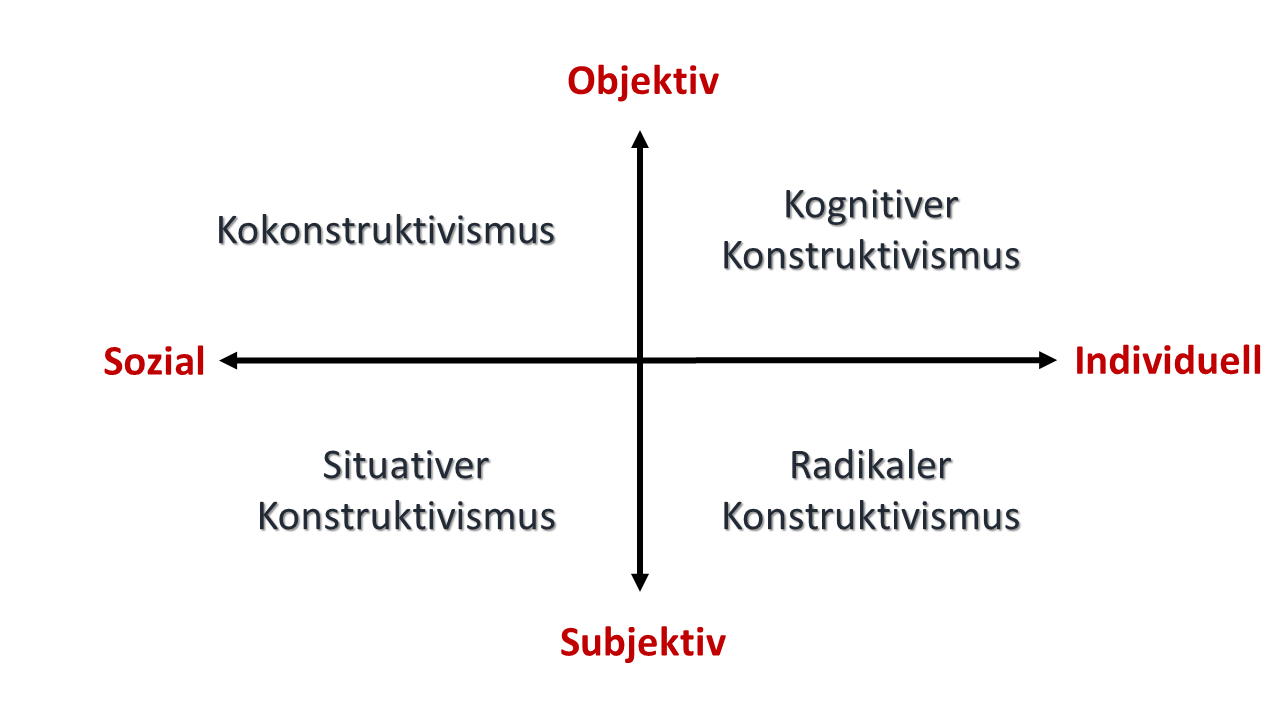
\includegraphics[width=1\textwidth]{Abbildungen/Anderson_1999_4positions.png}
	\caption{Die vier Ausrichtungen des Konstruktivismus nach \cite{Anderson.1999}.}
	\label{fig:Anderson.1999_4positions}
\end{figure}

Aus diesen zwei Dimensionen ergeben sich vier Ausrichtungen bzw. Ausprägungen des Konstruktivismus. 

Der \emph{Kognitive Konstruktivismus} zeichnet sich durch seine Betonung der Wichtigkeit von Konflikten und Unstimmigkeiten des konstruierten Wissens mit der tatsächlichen Realität für erfolgreiches Lernen aus. Nach \cite{Tobias.1991} sei es elementar, dass erworbenes und konstruiertes Wissen durch ständige Auseinandersetzung und Abgleich mit der Realität validiert und verbessert wird. 

Im Mittelpunkt des \emph{Radikalen Konstruktivismus} \label{par:konstr_pos_rad} steht die Auffassung welche auch \cite{Suchman.1987} teilt, dass keine gemeinsame Wahrnehmung aller Lernenden der Realität beim Lernen vorausgesetzt werden kann. Für eine Lernsituation in der von einem radikal konstruktivistischen Lernprozess ausgegangen wird, kann das Ergebnis des Lernens nicht mal im Ansatz vorausgesagt werden. Dies machte die Anregung zu Lernen durch den Lehrenden aber auch unmöglich, da er nicht weiß was seine Anregungen bewirken. \cite{Anderson.1999}

Genauso wie der Radikale Konstruktivismus geht auch der \emph{Situative Konstruktivismus} davon aus, dass es keine absolute Wahrheit gibt. \cite{Anderson.1999} Die beiden Ansätze unterscheiden sich aber dahingehend, dass dieser von einer sozialen Konstruktion von Wissen ausgeht. Das heißt, dass die Art und Weise, wie wir Dinge wahrnehmen darauf basiert, wie unser soziales Umfeld Dinge wahrnimmt. \cite{Jonassen.1992} %Beispielsweise nennt ein englischsprachig aufgewachsener Mensch einen Apfel "Apple" , da es das Umfeld genauso tut.

Der \emph{Kokonstruktivismus}, oder auch \emph{sozialer Konstruktivismus} genannt, geht auch wie der Situative Konstruktivismus davon aus, dass unser Umfeld beeinflusst, wie wir die Dinge wahrnehmen. Allerdings besteht der Unterschied darin, dass nach dem Kokonstruktivismus Diskussionen und soziale Interaktion zur Findung einer gemeinsamen Wahrheit führen. \cite{Bereiter.1994} Lernen in einem kokonstruktivistischen Lernprozess stellt den Lehrenden vor die Herausforderung, dass auch hier, ähnlich wie beim Radikalen Konstruktivismus (siehe \ref{par:konstr_pos_rad}), das Ergebnis des Lernen durch soziale Interaktion nicht eindeutig bestimmbar ist. \cite{Anderson.1999}
%\section{Ermöglichungsdidaktik}
%\label{sec:Ermoeglichungsdidaktik}

\section{Anwendung im E-Learning}
\label{sec:Konstr_Anwendungsfaelle}
Alex Koohang, Liz Riley und Terry Smith präsentieren in \cite[S. 95]{Koohang.2009} ein Modell zum Entwurf von E-Learnings, welches auf den Lernenden ausgerichtet ist. Begonnen wird ein solches E-Learning mit einer praktischen Problemsituation, welcher entweder vom Lehrenden oder angeregt durch diesen vom Lernenden entwickelt wird.
 
Unter Zuhilfenahme seiner Erfahrungen geht der Lernende die Problemsituation an und einen Lösungsvorschlag beziehungsweise eine Antwort. Dadurch wird gelernt. Die Ergebnisse werden in Gruppen und im Plenum diskutiert und bewertet. \cite[S. 95 - 96]{Koohang.2009}

Diese Kollaboration kann durch ein E-Learning-System unterstützt werden. Auch möglicherweise benötigte Informationen können über eine E-Learning-Plattform zur Verfügung gestellt werden. \cite[S. 96]{Koohang.2009} Die Aufbereitung des Themas für die Mitlernenden kann zur besseren Verknüpfung mit Erfahrungen im Gehirn des Lernenden führen. \cite[S. 101-102]{Koohang.2009}


	\chapter{Konnektivismus}
\label{cha:Konnektivismus}
Der Konnektivismus stellt die dritte und letzte Lerntheorie dar, welche im Rahmen dieser Arbeit vorgestellt wird. Georg Siemens doziert am Red River College in kanadischen Winnipeg und prägte die Lerntheorie 'Connectivism' (zu deutsch: Konnektivismus).\cite[S. 159]{Erpenbeck.2007}

\section{Definition}\label{Konnektivismus Definition}
Die heutzutage fortschreitende Vernetzung, basierend auf technologischen (Weiter-)Entwicklungen (bspw. das Internet) führt nach Siemens zu einer Veränderung des Lernens. Aus diesem Grund stellt er das Lernen mit Hilfe eines Netzwerkes in den Mittelpunkt. Der Konnektivismus ist eine recht junge Theorie, welche um das Jahr 2006 von Siemens veröffentlicht wurde. Er kritisiert die bis dahin existierenden Lerntheorien Behaviorismus, Kognitivismus (vgl. Kapitel \ref{cha:Kognitivismus}) sowie Konstruktivismus (Kapitel \ref{cha:Konstruktivismus}), da diese seiner Ansicht nach die heutzutage veränderten Rahmenbedingungen der Gesellschaft nicht ausreichend berücksichtigen.\cite[S.47 f.]{Kuhlmann.2008} 

Die 'alten' Lerntheorien suggerieren, dass Erfahrung eine zentrale Rolle im Lernprozess einnimmt. Aufgrund der durch die Digitalisierung geförderten Änderung der Lebens- und Arbeitsweisen, wird es immer schwieriger alle für den Lernprozess erforderlichen Informationsbestandteile sich durch Erfahrung anzueignen.\cite[S. 159ff.]{Erpenbeck.2007} Einige Gründe hierfür sind:
\begin{itemize}
	\item Eine zunehmende Vernetzung führt zur Informationsflut
	\item Der Lernende beschäftigt sich aufgrund wirtschaftlicher Gegebenheiten mit vielen verschiedenen (Theorie-)Bereichen
	\item Individuelle Lernbedürfnisse werden zunehmend relevanter
\end{itemize}
Basierend hierauf entwickelt Siemens den Konnektivismus als Lerntheorie, welche als Voraussetzung für die Aneignung von Wissen, den Aufbau sowie die Nutzung eines Netzwerkes sieht. Dieses besteht aus Personen, Organisation sowie Datenbanken, welche im weiteren Verlauf als Knoten bezeichnet werden. Somit beschreibt der Konnektivismus hauptsächlich den Lernprozess als den Aufbau und die Pflege dieses Netzwerkes, um stets für den Lernenden aktuelle sowie für eine Problemlösung adäquate Informationen zugänglich zu machen.

Er muss primär wissen, wo er welche Information findet. Diese muss nicht auswendig gekannt werden. Siemens formuliert darüber hinaus den Grundsatz, dass aktuelles Wissen wichtiger als persönliche Erfahrung ist. Nichtsdestotrotz beschreibt der Konnektivismus den Beitrag des Lernenden durch seine individuelle Erfahrungen, auch erlangt durch die Nutzung des Netzwerkes, sowie ebenfalls durch die Mitteilung von Wertevorstellungen, Emotionen, Denkhaltungen und Interaktion mit Netzwerkknoten als Lernprozess. Dies dient zur Aufrechterhaltung des in dieser Lerntheorie unabkömmlichen Netzwerkes und bildet die Basis für die Entwicklung neuer Erkenntnisse.

In diesem Modell nimmt der Lehrende hingegen zunehmend die Rolle des Mentors ein. Er gibt dem Lernenden unter anderem eine Hilfestellung bei der Einordnung des durch das Netzwerk zugänglichen Wissens.

Zusammenfassend kann gesagt werden, dass der Konnektivismus informelles sowie formelles Lernen miteinander vermischt.\cite[S. 47ff.]{Kuhlmann.2008} Die wird erreicht durch die Eingliederung von formellem Lernen (Nutzung von Bildungseinrichtungen für die Wissensaneignung \cite[S. 75]{Hellmer.2007}), sowie durch das Involvieren von informellem Lernen (Lernen im Alltag, ohne die Nutzung von pädagogischen Methoden. Hinzuziehen von Freunden, Familie, Bekannte \cite[S. 76]{Hellmer.2007}) in das oben beschriebene Netzwerk.  

\section{Anwendung im E-Learning}
Wie bereits in Abschnitt \ref{Konnektivismus Definition} erwähnt, nimmt die Individualisierung des Lernverhaltens zu. Dies führt zur vermehrten Nutzung von E-Learning und ist einer der Gründe, weshalb sich der Konnektivismus entwickelt hat.\cite[S. 47f.]{Kuhlmann.2008} Im folgenden sollen einige praktische Anwendungsempfehlung ausgesprochen werden, welche Lernen nach dieser Theorie unterstützen. Den Autoren dieser Arbeit erscheint der Einsatz von Kollaborationswerkzeugen in diesem Kontext besonders sinnvoll. 

Mit Hilfe eines Forums können Nachrichten mehreren Forum-Teilnehmern zugänglich gemacht, diskutiert, strukturiert sowie archiviert werden. Dies bietet den Vorteil Inhalte zu einem Thema zu sammeln und mit Hilfe der Teilnehmer, wie in Abschnitt \ref{Konnektivismus Definition} erwähnt, weiterzuentwickeln.\cite[S. 67f.]{Drummer.2011}

Eine weitere Möglichkeit der Kollaboration bietet der Einsatz eines Wikis, wie es bereits in Abschnitt \ref{sec:Konstr_Anwendungsfaelle} erläutert wurde. Der Vorteil des Wikis besteht in ihrer flexiblen Gestaltung hinsichtlich Struktur (Einbinden von Mitarbeiterverzeichnissen, Checklisten, Arbeitsanleitungen, Schulungsunterlagen uvm.) und lässt daher viele Anwendungsszenarien zu.\cite[S. 77]{Mertins.2009} Der Einsatz von Foren beschränkt sich gemäß der obigen Definition hauptsächlich auf Diskussionen.
	\chapter{Abschließende Bemerkung}
\label{cha:Schluss}
Im Folgenden werden diverse Unterschiede sowie Gemeinsamkeiten hinsichtlich der Rolle \emph{Lernender} sowie \emph{Lehrender} der drei Lerntheorie gegenübergestellt. Dabei wird auch, wie einleitend auf Seite \pageref{cha:Einleitung} erwähnt, eine aus der Autorensicht sinnvolle Zuordnung der didaktischen Modelle zur jeweiligen Theorie vorgenommen. 

Der Kognitivismus wie auch der Konstruktivismus sehen den Lernenden aktiv im Lernprozess involviert. Beide Theorien sprechen von der Verarbeitungsprozessen, welche im Inneren des Menschen beim Lernvorgang vonstatten gehen. Gerade der Kognitivismus legt wie in Abschnitt \ref{Definition Kognitivismus} näher erläutert, besonderes Augenmerk, und somit stärker als der Konstruktivismus, auf die Informationsverarbeitung während des Lernprozesses. Vergleicht man die beiden Lerntheorien bzgl. der Einflussnahme des Lehrenden auf den Lernerfolg, fällt auf, dass er in der kognitivistischen Lerntheorie größere Einflussnahme auf den Lernerfolg bzw. das Lernergebnis hat als im Konstruktivismus. Hier ist der direkte 1:1 Transfer des Wissens von Lehrende zu Lernende sehr viel schwieriger möglich, da Wissen in dieser Theorie beim Lernenden, wie Kapitel \ref{cha:Konstruktivismus} darlegt, individuell konstruiert wird. Dabei wird im Gegensatz zur kognitivistischen Theorie der Lehrende im Konstruktivismus oft als Berater, Coach oder auch Motivator beschrieben. \cite[S. 30ff.]{Bohm.2006} %FB sehr schön!

Möchte der Lehrende unter Berücksichtigung einer dieser beiden Lerntheorien ein Modell zur didaktischen Aufbereitung des Lernstoffs wählen, so ergibt aus Autorensicht folgende Zuordnung Sinn: Beide Theorien werden idealerweise mit dem didaktischen Modell der Anregung (vgl. \ref{sub:LernenDurchAnregung}) kombiniert. Dies begründet sich mit den in den Theorien verankerten Grundprinzipien der aktiven Auseinandersetzung des Lernenden im Lernprozess mit den Inhalten. Nur in besonderen Ausnahmefällen kann auf das Kopiermodell (vgl. \ref{sub:Kopiermodell}) bspw. bei der Vermittlung von Faktenwissen zurückgegriffen werden. Trotzdem gilt aufgrund neuer Erkenntnisse hinsichtlich verbesserte Lernerfolge durch Nutzung des Anregungsmodells, die Anwendung des Kopiermodells sofern möglich zu vermeiden.

Bei der Recherche für Informationen zum Konnektivismus fällt auf, dass die Einordnung dessen als Lerntheorie von einigen Autoren als kritisch eingestuft wird. Als Beispiel wird hierfür auf die von Kuhlmann und Sauter veröffentlichte Schrift \emph{Innovative Lernsysteme: Kompetenzentwicklung mit Blended Learning und Social Software} (vgl. \cite{Kuhlmann.2008}) sowie auf das von Gaby Filzmoser geschriebende Buch \emph{Bildungshaus 2.0} verwiesen. (vgl. \cite{Filzmoser.2013})

Kuhlmann und Sauter stufen den Konnektivismus nicht als Lerntheorie ein, da er ihrer Meinung nach die traditionellen Theorien erweitert und keine neuen Erkenntnisse hinsichtlich der Informationsverarbeitung durch den Menschen liefert. Der Konnektivismus sei ein pragmatischer Ansatz, welcher die in Abschnitt \ref{Konnektivismus Definition} erwähnten gesellschaftlichen Veränderungen berücksichtigt und als Lernkonzept formuliert .\cite[S. 50]{Kuhlmann.2008} 

Filzmoser bezieht sich auf Plon Verhagen, welcher als Professor für Educational Design an der Universität Twente lehrt und die Einstufung des Konnektivismus als Lerntheorie ebenfalls in Frage stellt. Seiner Meinung nach ist dieser eher Lernphilosphie als -theorie. Er gibt Verhagens Ansicht nach vorwiegend Antworten auf die Frage was gelernt wird und nicht wie gelernt wird.\cite[S. 26]{Filzmoser.2013}

Wie bereits in Abschnitt \ref{Konnektivismus Definition} auf Seite \pageref{RolleLernender} erläutert, ändert sich im Konnektivismus die Ansicht über den Prozess des Lernens. Aus diesem Grund steht nicht die interne Verarbeitung von Informationen im Vordergrund dieser Theorie, sondern hauptsächlich die aktive Interaktion mit Netzwerkknoten. Der Lernende nimmt somit genau wie im Kognitivismus und Konstruktivismus eine aktive, jedoch eine vorwiegend mit seinem Umfeld/Netzwerk dem Austausch gewidmete Rolle ein. Der Lehrende agiert, ähnlich wie im Konstruktivismus, als Coach. 

Die Zuordnung eines der erwähnten didaktischen Aufbereitungsmodelle ist aus Sicht der Autoren für diese Theorie, aufgrund der von verschiedenen Autoren genannten Zweifel zur Einstufung als diese, schwierig. Darüber hinaus wird der Lernprozess vorwiegend als Netzwerkpflege und -ausbauaufgabe gesehen, was die Zuordnung einer der didaktischen Modelle weiter erschwert. Dennoch soll sich nach Meinung der Autoren dieser Arbeit der Lernende idealerweise durch Anregung mit anderen Netzwerkknoten, gerade für die Weiterentwicklung von Wissen, austauschen. Hierbei empfiehlt sich ähnlich dem Anregungsmodell (siehe \ref{sub:LernenDurchAnregung}) vorzugehen.

Eine tabellarische Zusammenfassung mit den in dieser Arbeit abgegebenen Handlungsempfehlung für die jeweilige Lerntheorie kann dem Anhang auf Seite \pageref{fig:Unterschiede und Handlungsempfehlungen für die Lerntheorien} entnommen werden. 


 
	
	\clearpage
	
	% Ab hier weiter mit großen, römischen Seitenzahlen
	\pagenumbering{Roman}
	
	% Seitenzähler auf zwischengespeicherten Wert für große, römische Zahlen setzen
	\setcounter{page}{\theRomanPagenumber}

	% Kopf links auf Titel ändern
	\ihead[\titel]{\titel}	
	
	% Anhang
	%\addchap{Appendices}
	
	\appendix
	\chapter{Anhang}
\newpage
\section{Unterschiede und Handlungsempfehlungen für die Lerntheorien in der Übersicht}
\begin{figure}[h]
	\centering
	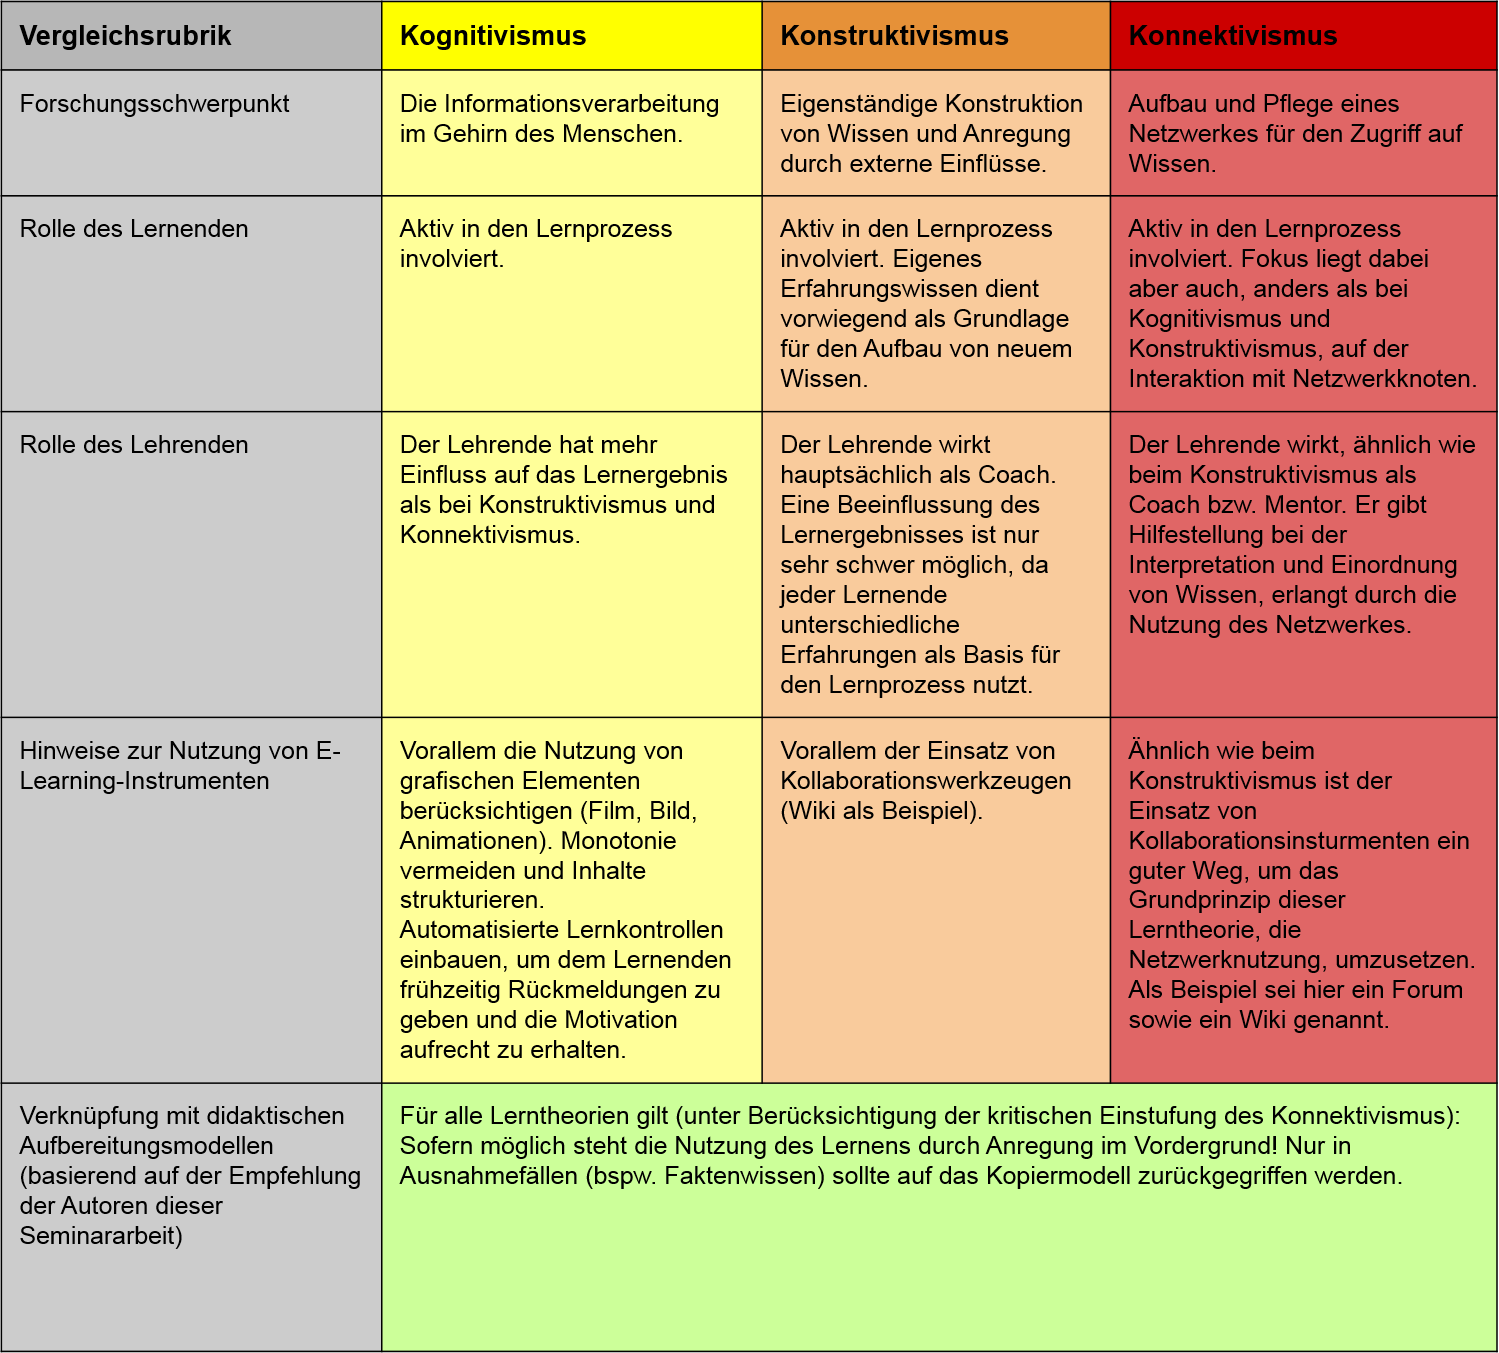
\includegraphics[width=1.0\textwidth]{Abbildungen/Gegenuberstellung.png}
	\caption{Unterschiede und Handlungsempfehlungen für die Lerntheorien in der Übersicht. Eigene Darstellung basierend auf den Inhalten dieser Arbeit.}
	\label{fig:Unterschiede und Handlungsempfehlungen für die Lerntheorien}
\end{figure}
	
	% Beigaben
	%\addchap{Beigaben}
\label{cha:Beigaben}

Im Folgenden ist die Verzeichnisstruktur der beigelegten CD dargestellt.
 
\begin{description}
	\item[Abbildungen]
		Beinhaltet die verwendeten Abbildungen.
	\item[Literatur]
		Beinhaltet das Literaturverzeichnis im \textit{\BibTeX{}} Format, sowie die digital verfügbaren Quellen als \textit{PDF} oder \textit{MHT}.
	\item[Seminararbeit]
		Beinhaltet die Seminararbeit als \textit{PDF}.
		Der zugehörige \emph{\LaTeX{}} Source Code befindet sich im Unterverzeichnis \textit{LaTeX}.
		Im Unterverzeichnis \textit{DOC} befindet sich die von \textit{PDF} in \textit{DOC} konvertierte Version dieser Arbeit.
\end{description}
	
	% Literaturverzeichnis
	
	\printbibliography	
	% Aktuellen Abschnitt beenden
	\clearpage
\end{document}